\documentclass[conference]{IEEEtran}
\usepackage[backend=biber, style=ieee]{biblatex}  % Use IEEE style for references
\addbibresource{references.bib} % Included references file
\IEEEoverridecommandlockouts
% The preceding line only needs to identify funding in the first footnote. If that is unnecessary, please comment on it.
% \usepackage{cite}
\usepackage{amsmath,amssymb,amsfonts}
\usepackage{algorithmic}
\usepackage{graphicx}
\usepackage{textcomp}
\usepackage{xcolor}
\usepackage{tikz}
\usetikzlibrary{shapes.geometric, arrows}

\tikzstyle{startstop} = [rectangle, rounded corners, minimum width=2cm, minimum height=1cm, text centered, draw=black, inner sep=2pt]
\tikzstyle{process} = [rectangle, minimum width=2.5cm, minimum height=1cm, text centered, draw=black, inner sep=2pt]
\tikzstyle{arrow} = [thick,->,>=stealth]

% \def\BibTeX{{\rm B\kern-.05em{\sc i\kern-.025em b}\kern-.08em
%     T\kern-.1667em\lower.7ex\hbox{E}\kern-.125emX}}
\begin{document}

\title{Estimating Motion Uncertainty in Vehicles\\
}

\author{\IEEEauthorblockN{Aarya Gupta, Aditya Raj Jain, Aditya Kumar Singh}

\IEEEauthorblockA{\textit{Networked Autonomous Systems Lab IIITD} \\
\textit{Indraprastha Institute of Information Technology}\\
Delhi, India \\
\{aarya22006, aditya22037, aditya22598\}@iiitd.ac.in}
}

\maketitle

\begin{abstract}
Predictive capabilities and decision-making processes bind every Autonomous vehicle's safety.\\ Probabilistic prediction varies depending on real-life factors. It can be divided into Aleatory(stochastic) and epistemic(non-stochastic). \\
This project aims to analyse various methods to improve the protective capabilities of an uncomplicated kinematic bicycle's steering angle prediction model.\\
We primarily compare and combine the KDE (Kernel Density Function) and Bootstrapping to predict the next angle while using Bayesian updation (Maximum A posteriori) to improve the model with the obtained data of previous iterations.
\end{abstract}

\begin{IEEEkeywords}
Autonomous vehicles, Kinematic bicycle model, Aleatory uncertainty
Epistemic uncertainty, Kernel Density Estimation (KDE),
Bootstrapping, Maximum A posteriori (MAP)
\end{IEEEkeywords}

\section{Introduction}
The system operates under the following assumptions:

\begin{enumerate}
    \item \textbf{Discrete Time System}: The system is modelled as a discrete-time system.
    \item \textbf{Uniform Time Increments}: Time increments are fixed, with $\Delta t = 1$.
    \item \textbf{Underlying System Equations}: The bicycle model in our world follows the following equations:

    \begin{subequations}
    \renewcommand{\theequation}{1\alph{equation}}
    \begin{equation}
    \theta(t) = \theta(t-\Delta t) + \Delta \theta(t)
    \end{equation}
    \begin{equation}
    x(t) = x(t-\Delta t) + v \cdot \cos(\theta(t)) \cdot \Delta t
    \end{equation}
    \begin{equation}
    y(t) = y(t-\Delta t) + v \cdot \sin(\theta(t)) \cdot \Delta t
    \end{equation}
    \end{subequations}
    Here, 
    \begin{itemize}
        \item $\theta$ is the R.V. describing the heading angle of the vehicle.
        \item $\Delta\theta$ is the R.V. describing the change in heading angle.
        \item $x$ and $y$ are the R.V.s depicting the position.
    \end{itemize}

    \item \textbf{Initial Conditions and Assumptions}:
    \begin{itemize}
        \item Let the true underlying (unknown) distribution of $\Delta\theta(t)$ be $\hat{\mathcal{F}}$, which is same for all time instants.
        \item Values of $x_0$, $y_0$, $\theta_0$, $v$ are definite/constants and are given.
        \item For simplicity, let's assume $x_0$, $y_0$, $\theta_0$ to be 0 while the vehicle is moving with a constant speed of 1.
        \begin{equation}
        \Rightarrow \theta_0 = 0, \quad \Delta\theta_0 = 0, \quad x_0 = 0, \quad y_0 = 0, \quad v = 1
        \end{equation}
        \item Assuming the initial set of values $\mathcal{F}_{1}$ are given, from which $\Delta \theta_1$ will chose a value. $\mathcal{F}_{1}$ represents the distribution of $\Delta \theta_1$.
    \end{itemize}
    
\end{enumerate}

% \begin{table}[h!]
%     \centering
%     \small  % Reduce font size to fit the table within the column width
%     \begin{tabular}{|c|c|c|c|c|}
%         \hline
%         & $t=0$ & $t=1$ & $t=2$ & $t=3$ \\
%         \hline
%         Known RVs & \parbox[c]{2.5cm}{$\theta_0=0$, $\Delta \theta_0 = 0$ \\ $x_0=0$, $y_0=0$ \\ $\mathcal{F}_{1}$ $(\Delta \theta_1$ distrib.)}  & \parbox[c]{2.4cm}{$\Delta \theta_1$ (observed) \\ $\theta_1$, $x_1$, $y_1$} & \parbox[c]{2.4cm}{$\Delta \theta_2$ (observed) \\ $\theta_2$, $x_2$, $y_2$} & \parbox[c]{2.4cm}{$\Delta \theta_3$ (observed) \\ $\theta_3$, $x_3$, $y_3$}\\
%         \hline
%         Predicted RVs & - & $\mathcal{F}_{2}$ $(\Delta \theta_2$ dist.) & $\mathcal{F}_{3}$ $(\Delta \theta_3$ dist.) & $\mathcal{F}_{4}$ $(\Delta \theta_4$ dist.) \\
%         \hline
%     \end{tabular}
%     \vspace{0.2cm}  % Adjust vertical space as needed
%     \caption{System Timeline}
%     \raggedright
%     \label{tab:sample_table}
% \end{table}

% Table with columns till t=2 so that the table can be inserted entirely into the page.
\begin{table}[h!]
    \centering
    \renewcommand{\arraystretch}{1.75} % Adjust the value to increase or decrease the vertical spacing
    \small  % Reduce font size to fit table within column width
    \begin{tabular}{|c|c|c|c|}
        \hline
        & $t=0$ & $t=1$ & $t=2$ \\
        \hline
        Known RVs & \parbox[c]{2.25cm}{\centering $\theta_0=0$, $\Delta \theta_0 = 0$ \\ $x_0=0$, $y_0=0$ \\ $\mathcal{F}_{1}$ $(\Delta \theta_1$ distrib.)}  & \parbox[c]{2.35cm}{\centering $\Delta \theta_1$ (observed) \\ $\theta_1$, $x_1$, $y_1$} & \parbox[c]{2.35cm}{\centering $\Delta \theta_2$ (observed) \\ $\theta_2$, $x_2$, $y_2$} \\
        \hline
        Predicted RVs & - & $\mathcal{F}_{2}$ $(\Delta \theta_2$ distr.) & $\mathcal{F}_{3}$ $(\Delta \theta_3$ distr.) \\
        \hline
        \parbox[c]{1.8cm}{\centering True Distrib.\\ (Unknown)} & $\hat{\mathcal{F}}$ & $\hat{\mathcal{F}}$ & $\hat{\mathcal{F}}$ \\
        \hline
    \end{tabular}
    \vspace{0.2cm}  % Adjust vertical space as needed
    \caption{System Timeline}
    \raggedright
    $\mathcal{F}_{t}$ is the predicted distribution at time $t-1$ from $\mathcal{F}_{t-1}$ $\forall$ $t \geq 2$. The true value of $\Delta \theta_t$ at $t$ will be observed from the true unknown distribution $\hat{\mathcal{F}}$.
    \label{tab:sample_table}
\end{table}

To estimate the underlying distribution of $\Delta \theta$, the following approached are followed:
\subsection{Kernel Density Estimation (KDE)}
Imagine you have a bunch of data points, and you want
to understand their distribution. Kernel Density Estimation
(KDE) is like a sophisticated way of creating a smooth
curve that represents this distribution by placing a curve (Kernel) at all the points from the sample and adding them up to find the distribution (It is normalised such that probability adds up to 1). It’s particularly useful when you don’t know the underlying shape of your data’s distribution.

\subsection{Bootstrapping}
Initially, given a set of real-world samples, we create bootstrap samples at each time step by randomly selecting elements from the original set, allowing replacement. The predicted distribution at each time step is the bootstrapped distribution of the original set. The true value of the change at each time step is observed from this predicted distribution. We calculate the Mean Squared Error (MSE) at each time step to understand the underlying distribution of changes over time. This MSE is measured between the predicted and initial real-world data distributions. We aim to minimize this MSE as time progresses, indicating that our predictions are becoming more accurate and approaching the unknown underlying distribution.



\subsection{KDE combined with Bootstrapping}
In this, we combine the benefits of KDE and bootstrapping. From the original samples, we bootstrap it to produce 500 samples. For each sample, we construct a KDE distribution. All the samples are assigned a different kernel bandwidth. Finally, all the distributions are combined to form a final distribution, with a bandwidth normalised from all the samples. It increases the computational complexity but provides a better estimate of the underlying distribution.

\subsection{Bayesian Updation}
This is a statistical method to update our prior distribution based on new observed data through the help of Bayes' theorem.\\
Over time, it has the capability to predict the underlying distribution accurately given certain constraints.

\section{Introduction to Kernel Density Estimation (KDE)}

\subsection{Basic Idea}

KDE places a small "bump" (called a kernel) at each data point and then adds up all these bumps to create a smooth curve. This curve estimates the probability density function (PDF) of your data.

\subsection{Mathematical Formulation}

The kernel density estimator is defined as:

\begin{equation}
    \hat{f}_h(x) = \frac{1}{nh} \sum_{i=1}^n K\left(\frac{x - X_i}{h}\right)
\end{equation}

Here, $\hat{f}_h(x)$ is our estimated density at point $x$, $n$ is the number of data points, $h$ is the bandwidth (which controls how wide our bumps are), $K$ is the kernel function (the shape of our bumps), and $X_i$ are our individual data points.

\subsection{Kernel Functions}

The kernel function $K$ determines the shape of our bumps. It must integrate to 1 over its domain:

\begin{equation}
    \int_{-\infty}^{\infty} K(u) du = 1
\end{equation}

Standard kernel functions include:

1. Gaussian (Normal) Kernel:
\begin{equation}
    K(u) = \frac{1}{\sqrt{2\pi}} e^{-\frac{1}{2}u^2}
\end{equation}

This is like using little bell curves as our bumps.

2. Epanechnikov Kernel:
\begin{equation}
    K(u) = \frac{3}{4}(1-u^2) \text{ if } |u|\leq 1, \text{ else } 0
\end{equation}

This uses parabolic bumps, which some consider optimal in a mathematical sense.

\section{The Math Behind KDE}

\subsection{Bias-Variance Tradeoff}

In statistics, we often deal with a tradeoff between bias (how far off our estimate is on average) and variance (how much our estimate varies with different samples). KDE is no exception.

The mean integrated squared error (MISE) helps us quantify this tradeoff:

\begin{equation}
    \text{MISE}(\hat{f}_h) = \int (\text{Bias}[\hat{f}_h(x)])^2 dx + \int \text{Var}[\hat{f}_h(x)] dx
\end{equation}

Considering both bias and variance, this equation tells us how good our estimate is overall.

\subsection{Bandwidth Selection}

Choosing the proper bandwidth $h$ is crucial. Too small, and our estimate will be too spiky; too large, and it will be too smooth, missing essential features.

The optimal bandwidth that minimizes the asymptotic MISE is:

\begin{equation}
    h_{opt} = \left(\frac{R(K)}{n \mu_2(K)^2 R(f'')}\right)^{1/5}
\end{equation}

where $R(K) = \int K^2(u) du$, $\mu_2(K) = \int u^2 K(u) du$, and $R(f'') = \int (f''(x))^2 dx$.

In practice, we often use data-driven methods like cross-validation to choose $h$.

\subsection{Multivariate KDE}

When dealing with multiple variables (like position and velocity), we use multivariate KDE:

\begin{equation}
    \hat{f}_H(x) = \frac{1}{n} \sum_{i=1}^n K_H(x - X_i)
\end{equation}

Here, $H$ is a matrix that determines the width and orientation of our multidimensional bumps.

\section{Applying KDE to Your Data}

To use KDE on your incoming data:

1. Collect your data points (e.g., steering angles and accelerations).
2. Choose a kernel function (Gaussian is a good start).
3. Select a bandwidth (you can use cross-validation or a rule of thumb).
4. Apply the KDE formula to estimate the probability density.

This gives you a smooth estimate of the probability distribution of your data, which you can use for further analysis or prediction.

\section{Bootstrapping}
\subsection{Bootstrapping the Samples}

Given a set of real-world samples \( \{x_1, x_2, \ldots, x_n\} \), each bootstrap sample \(\mathbf{X}_i^*\) is defined as \( \{x_{i1}^*, x_{i2}^*, \ldots, x_{in}^*\} \) is obtained by randomly sampling from the original set with replacement. 
% We repeat this process 500 times to create 500 bootstrap samples \( \{X_1^*, X_2^*, \ldots, X_{500}^*\} \).


\subsection{Implying the above logic in our system (Refer to Table 1)}
% $\mathcal{F}_{t}$ is the bootstrapped distribution at time $t-1$ from $\mathcal{F}_{t-1}$ $\forall$ $t \geq 2$. The true value of $\Delta \theta_t$ at $t$ will be observed from the predicted $\mathcal{F}_{t}$ at t-1.

$\mathcal{F}_{t}$ is the bootstrapped distribution at time $t-1$ from $\mathcal{F}_{1}$ $\forall$ $t \geq 1$. The true value of $\Delta \theta_t$ at $t$ will be observed from the predicted $\mathcal{F}_{t}$ at t-1. \\
To reach the underlying distribution of $\Delta \theta_t$, we will find the \textbf{Mean Square Error} at time t defined as $\textbf{MSE}_\textbf{t}$, between predicted $\mathcal{F}_{t+1}$ \& $\mathcal{F}_{1}$; and we will try to minimise this MSE as time progresses.

The $\text{MSE}_{t}$ between two distributions (lists of values) $\mathcal{F}_{1}$ (given real-world data) \( \{x_1, x_2, \ldots, x_n\} \) and $\mathcal{F}_{t+1}$ \( \{\hat{x}_{t+1,1}, \hat{x}_{t+1,2}, \ldots, \hat{x}_{t+1,n}\} \) (data predicted at time t) is defined as:

\begin{subequations}
    \begin{equation}
    \text{MSE}_{t} = \frac{1}{n} \sum_{i=1}^{n} (x_i - \hat{x}_{t+1, i})^2
    \end{equation}
\end{subequations}

The aim is to minimise this MSE, and take it to below some predefined threshold value $\text{MSE}_{min}$ so that for some t, $\mathcal{F}_{t+1}$ is the distribution nearest to the unknown underlying distribution. 

\textcolor{red}{More information to be added } 


\section{KDE combined with Bootstrapping}


\subsection{Creating KDE Distributions with Varying Bandwidths}
Once we have the bootstrapped samples, we create a KDE for each sample. The bandwidth of the KDE determines the smoothness of the estimated density. We explore two methods for selecting the bandwidth:

\subsection{Method 1: Assigning a Linear Range of Bandwidths}
In this method, we assign bandwidths to each KDE in a linearly increasing manner. Specifically, for the \( i \)-th bootstrapped sample, we set the bandwidth \( h_i \) as:
\[
h_i = \frac{c(i - 1)}{499}, \quad \text{for } i = 1, 2, \ldots, 500
\]
This means the first KDE has a bandwidth of 0, and the last has a bandwidth of c. Where c is decided based on samples. \\
\textcolor{red}{Add information about the silverman and scott's rule and why this may be better than those}

\subsection{Method 2: Using the Standard Deviation as Bandwidth}
In the second method, we use the standard deviation of each bootstrapped sample as the bandwidth. For the \( i \)-th bootstrapped sample \( X_i^* \), the bandwidth \( h_i \) is:
\[
h_i = \text{std}(X_i^*)
\]
where \( \text{std} \) denotes the standard deviation of the sample \(X_i^*\)

\subsection{Combining KDE Distributions}
We average the estimated densities to create a final KDE distribution from the 500 individual KDEs. If \( f_i(x) \) is the KDE for the \( i \)-th bootstrapped sample with bandwidth \( h_i \), the final combined KDE \( f(x) \) is:
\[
f(x) = \frac{1}{500} \sum_{i=1}^{500} f_i(x)
\]
Each \( f_i(x) \) is given by:
\[
f_i(x) = \frac{1}{n h_i} \sum_{j=1}^{n} K \left( \frac{x - x_j^*}{h_i} \right)
\]
where \( K \) is the kernel function, typically a Gaussian function:
\[
K(u) = \frac{1}{\sqrt{2\pi}} e^{-\frac{u^2}{2}}
\]

\section{Bayesian Inference}
When we have an existing distribution, and new data becomes available, we can update the existing distribution to reflect the latest information using Bayesian updating. 
\subsection{Bayesian inference}
Given some observed data, this method provides a strong theoretical framework to predict the underlying probability distribution.\\
\begin{enumerate}
\item We assume a prior distribution. Since we don't want to make any assumptions, we assume a uniform distribution. 
\[
\theta \sim U(0,1)
\]
\item Suppose we have some experimental data from the original underlying distribution. We wish to update our current understanding of the PDF on the basis of this new information. \\
We first calculate the likelihood (\( p(D | \theta)) \) where \( p(\theta) \) is the prior distribution and \( D = \{x_1, x_2, \ldots, x_n\} \) is the observed data.\\
\item Next, we calculate \( p(D) \) i.e. probability of observed data independent of \(\theta\) using the formula \[
p(D) = \int_{0}^{1} p(A | \theta) f(\theta) d\theta
\]

\item Now, using the Bayes rule, we can update the priori distribution based on the new data such that
\[
p(\theta | D) \propto \frac{p(D | \theta) p(\theta)}{p(\theta)}
\]
\end{enumerate}
From this, we can find posterior distribution, which can be used to predict future probabilities and can be updated using new original data observed at each time step.\\
Though this method is quite robust and easy to use, it is Parametric, i.e. it assumes a prior distribution to work with (Uniform in this case). If the initial distribution is very different from the underlying distribution, it may take a long time to reach the correct underlying distribution.

\subsection{Updating the KDE Distribution}
Suppose we have an initial KDE distribution \( f_{prior}(x) \) representing our prior knowledge of the distribution. After observing new data \( D = \{x_1, x_2, \ldots, x_n\} \), we can update this distribution using MAP estimation.
\begin{enumerate}

\item Construct the Likelihood: Assume the observed data \( D \) follows the KDE distribution \( f_{prior}(x) \). The likelihood \( p(D | f_{prior}) \) can be constructed from the KDE's evaluation on the new data points.

\item Update the Prior: Combine the prior KDE with the likelihood to get the posterior KDE. We achieve this by adjusting the KDE to incorporate the new data points. This can be done by re-estimating the KDE with the latest data added to the original dataset or by weighting the prior and new KDEs.

\item Find the MAP Estimate: The MAP estimate in this context is the updated KDE that maximizes the posterior distribution.
\end{enumerate}
% \newpage
\section{REVISED METHODOLOGY}

The aforementioned approaches, which consider discrete time instants, are found to be inefficient for predicting the underlying distribution. Consequently, we propose a modified approach. Assume we are given the true values of $\Delta\theta$ observed during the vehicle's motion. We aim to determine the true underlying distribution of the random variable $\Delta\theta$, once the vehicle's motion has been completed and the set of true $\Delta\theta$ values has been obtained. To achieve this, we will employ the previously discussed techniques, namely Kernel Density Estimation (KDE), Bootstrapping, and a combination of KDE with Bootstrapping, to ascertain the underlying distribution from the provided data sample.

\subsection{Initial Conditions and Assumptions}
\begin{itemize}
    \item Let the true underlying (unknown) distribution of $\Delta\theta(t)$ be denoted as $\mathcal{F}$. Let the true unknown mean be represented as $\theta$.
    \item Let there be an empirical distribution $\hat{\mathcal{F}}$ representing the set of true $\Delta\theta$ values obtained once the vehicle's motion has been completed. Let the mean of this empirical distribution be $\hat{\theta}$, serving as the plug-in estimate.
    
\end{itemize}



\section{ESTIMATING UNCERTAINTY WITH CONFIDENCE INTERVALS}
Confidence intervals provide a range of values within which we expect the true population parameter (true mean in this case) to lie, giving us a measure of uncertainty and reliability about our sample estimates. To find the most reliable confidence interval, we will try out 5 different approaches, which assume the underlying true distribution to be some distribution, and then provide a confidence interval.
Finding the confidence interval, assuming the true underlying distribution to be:

\subsection{Standard Normal}
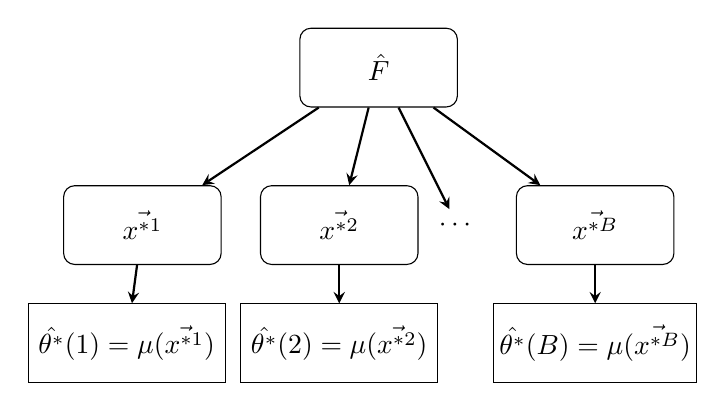
\begin{tikzpicture}[node distance=1.5cm]

% Root node
\node (F) [startstop] {$\hat{F}$};

% First row nodes
\node (x1) [startstop, below of=F, xshift=-3cm, yshift=-0.5cm] {$\vec{x^{*1}}$};
\node (x2) [startstop, below of=F, xshift=-0.5cm, yshift=-0.5cm] {$\vec{x^{*2}}$};
\node (dots) [text centered, below of=F, xshift=1cm, yshift=-0.5cm] {$\cdots$};
\node (xB) [startstop, below of=F, xshift=2.75cm, yshift=-0.5cm] {$\vec{x^{*B}}$};

% Second row nodes
\node (theta1) [process, xshift=-0.2cm, below of=x1] {$\hat{\theta^*}(1) = \mu(\vec{x^{*1}})$};
\node (theta2) [process, below of=x2] {$\hat{\theta^*}(2) = \mu(\vec{x^{*2}})$};
\node (thetaB) [process, below of=xB] {$\hat{\theta^*}(B) = \mu(\vec{x^{*B}})$};

% Drawing arrows
\draw [arrow] (F) -- (x1);
\draw [arrow] (F) -- (x2);
\draw [arrow] (F) -- (dots);
\draw [arrow] (F) -- (xB);
\draw [arrow] (x1) -- (theta1);
\draw [arrow] (x2) -- (theta2);
\draw [arrow] (xB) -- (thetaB);

\end{tikzpicture}
\\  \\
In the above chart, 
\begin{itemize}
    \item $\hat{F}$ represents the empirical distribution given to us.
    \item {$\vec{x^{*i}}$} represents the $i$-th bootstrap sample $\forall i \in [1, B]$; (resampled with replacement from the given data).
    \item $\hat{\theta^*}(i)$ represents the bootstrap replication of $\hat{\theta}$; 
    \item The mean of the given population (plug-in estimate) is represented as $\hat{\theta}$ s.t. $\hat{\theta} = \mu(\hat{F}) $.
\end{itemize}

Now, find the standard error associated with the means of the bootstrapped samples.\\

$\hat{\text{se}_B} $ = $\sqrt{\frac{1}{B-1} \sum_{b=1}^{B} \left( \hat{\theta^*}(b) - \hat{\theta^*(.)} \right)^2 }$
 \\where,
$\hat{\theta^*(.)} $ = ${\frac{1}{B} \sum_{b=1}^{B} \left( \hat{\theta^*}(b) \right)^2 }$ \\

The confidence interval can be written as:
\[
\hat{\theta} \pm Z^{(1-\alpha)} \cdot \hat{\text{se}}_B
\]


\[
\implies \theta \in \left[ \hat{\theta} - Z^{(1-\alpha)} \cdot \hat{\text{se}}_B, \; \hat{\theta} - Z^{\alpha} \cdot \hat{\text{se}}_B \right]
\]

where, $\newline$
$\hat{Z}^{(1-\alpha)} = -\hat{Z}^{\alpha}$ $\newline$
$\hat{Z}^{\alpha}$ represents the 100.$\alpha^{th}$ percentile point of N(0, 1) distribution. $\newline$
$\hat{\theta}$ represents the plug-in estimate (the sample's mean).$\newline$
$\theta$ represents the true mean of the underlying distribution.

% Practical Application:
% Insert the image
\begin{figure}[h] % The [h] option places the figure approximately here
    \centering % Center the image
    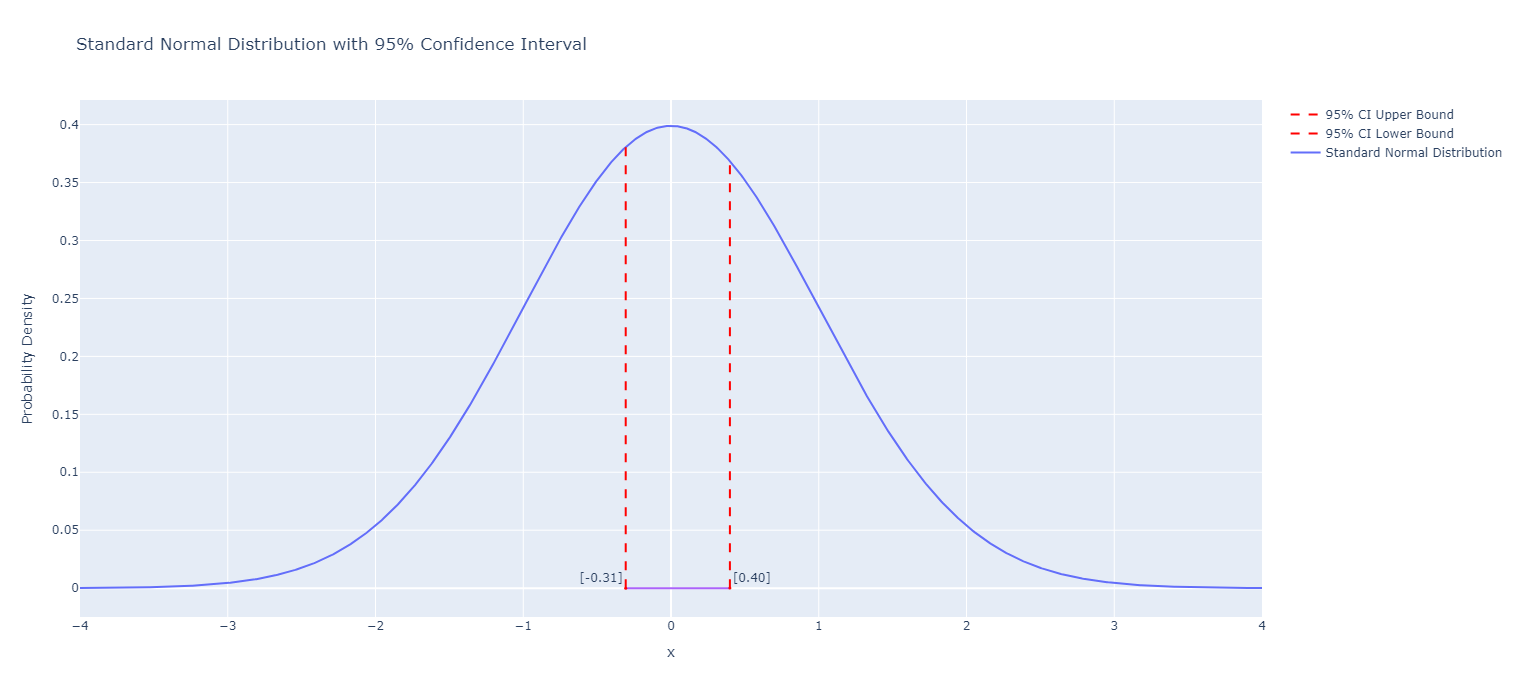
\includegraphics[width=0.65\textwidth]{normal.png} % Adjust the width as needed
    \caption{Confidence Intervals (95\% confidence) showing the uncertainity of the true mean.} % Caption for the image
    \label{fig:example_graph} % Label for referencing the image
\end{figure}

\newpage
\subsection{Student-t}
All the calculation remain same as done in Section IX-A. The assumed underlying distribution in this case will be student-t distribution. By using this, we induced the notion of known mean and unknown variance; different from the case of known mean and variance in standard normal. 


The confidence interval can be written as:
\[
\hat{\theta} \pm t^{1-\alpha} \cdot \hat{\text{se}}_B
\]


\[
\implies \theta \in \left[ \hat{\theta} - t^{(1-\alpha)} \cdot \hat{\text{se}}_B, \; \hat{\theta} - t^{\alpha} \cdot \hat{\text{se}}_B \right]
\]

where, $\newline$
$\hat{t}^{(1-\alpha)} = -\hat{t}^{\alpha}$ $\newline$
$\hat{t}^{\alpha}$ represents the 100.$\alpha^{th}$ percentile point of bootstrap-t distribution. $\newline$
$\hat{\theta}$ represents the plug-in estimate (mean of the given sample).$\newline$
$\theta$ represents the true mean of the underlying distribution.


% Practical Application:
% Insert the image
\begin{figure}[h] % The [h] option places the figure approximately here
    \centering % Center the image
    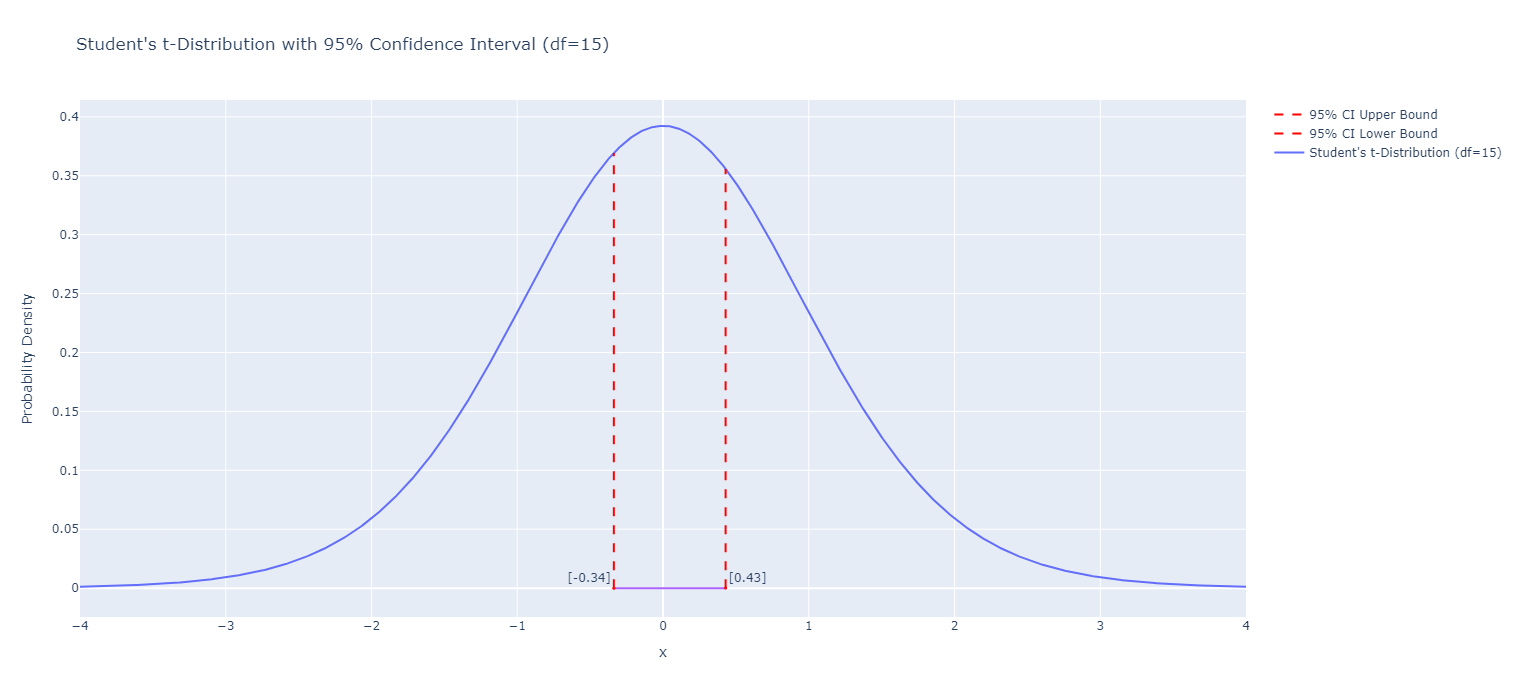
\includegraphics[width=0.65\textwidth]{student-t-df_15.png} % Adjust the width as needed
    \caption{Confidence Intervals (95\% confidence) showing the uncertainity of the true mean \{degrees of freedom = 15\}}. % Caption for the image
    \label{fig:student-t_graph_df_15} % Label for referencing the image
\end{figure}


\subsection{Bootstrap-t}


\subsection{Percentile Method}


\subsection{BCa (Bias-corrected and accelerated}


\section*{Conclusion}

\textcolor{red}{Add conclusion}

\cite{efron1994introduction}
\cite{edition2002probability}
\printbibliography
\end{document}

